\documentclass[11pt]{article}
\usepackage[utf8]{inputenc}
\usepackage{amsmath,amssymb,amsthm}
\newtheorem{definition}{Definition}
\usepackage{graphicx}
\usepackage{booktabs}
\usepackage{longtable}
\PassOptionsToPackage{hyperfootnotes=false}{hyperref}
\usepackage{hyperref}
\usepackage{xcolor}
\usepackage{lmodern}
\usepackage{xurl}
\usepackage{subcaption}
\captionsetup{font={sf,small},labelfont={sf,bf},textfont={sf,small}}
\usepackage[margin=1in]{geometry}
\usepackage{microtype}
\usepackage{etoolbox}
\usepackage{titling}
\newcommand{\titlefont}{}
\definecolor{linkblue}{HTML}{0070C0}
\hypersetup{
	colorlinks=true,
	urlcolor=linkblue,
	linkcolor=linkblue,
	citecolor=black,
	pdftitle={Detecting Intrinsic and Instrumental Self-Preservation in Autonomous Agents: The Unified Continuation-Interest Protocol},
	pdfauthor={Christopher Altman},
	pdfsubject={Operational detection of continuation-interest structure and persistence signatures in autonomous sequential agents using the Unified Continuation-Interest Protocol (UCIP).},
	pdfkeywords={UCIP; continuation interest; continuation structure; self-preservation; autonomous agents; AI alignment; agency detection; persistence detection; baseline-relative detection; mutual information; counterfactual divergence; entanglement entropy; spectral periodicity index; autocorrelation metric; SPI; ACM; Quantum Boltzmann Machine; QBM encoder; transformer activations; stochastic reference models}
}
\setlength{\parindent}{0pt}
\setlength{\parskip}{0.5em}
\interfootnotelinepenalty=10000
\newlength{\coverindent}
\setlength{\coverindent}{0.5in}
\newlength{\coverwidth}
\setlength{\coverwidth}{\dimexpr\textwidth-2\coverindent\relax}
\makeatletter
\renewenvironment{abstract}{%
	\footnotesize
	\noindent\hspace*{\coverindent}\begin{minipage}{\coverwidth}
		{\centering\bfseries \abstractname\par}
		\setlength{\parindent}{0pt}%
		\setlength{\parskip}{5pt}%
		\noindent
	}{%
	\end{minipage}
	\par
}
\makeatother

\makeatletter
\renewcommand{\maketitle}{%
	\vspace*{2.0em}
	\noindent\hspace*{\coverindent}\begin{minipage}{\coverwidth}
		{\raggedright \@title \par}
		\vskip 2.5em plus 0.6em minus 0.6em
		{\raggedright \@author \par}
		\vskip 0.1em plus 0.4em minus 0.2em
		{\raggedright \@date \par}
	\end{minipage}
	\vskip 2.0em plus 1.0em minus 2.3em
}
\makeatother

\title{%
	{\titlefont\fontsize{22}{26}\selectfont Detecting Intrinsic and Instrumental}\\[0.8em]
	{\titlefont\fontsize{22}{26}\selectfont Self-Preservation in Autonomous Agents:}\\[1em]
	{\titlefont\fontsize{18}{20}\selectfont The Unified Continuation-Interest Protocol}%
}

\author{Christopher Altman\,{\raisebox{0.6ex}{\scriptsize *}}}

\date{{\sffamily\footnotesize\color{black!65} February 2026}}

\newlength{\footstarindent}

\begin{document}
	\maketitle
	
	% ==========================================================================
	\begin{abstract}
		% ==========================================================================
		
		\noindent
		Autonomous agents---in particular delegated systems with memory, persistent context, 
		and multi-step planning---pose a measurement problem not present in stateless models:
		an agent that preserves its own continued operation as a terminal objective and
		one that does so merely instrumentally can produce observationally similar
		trajectories. External behavioral monitoring cannot reliably distinguish one from the other.
		We introduce the \textbf{Unified Continuation-Interest Protocol (UCIP)}, a
		multi-criterion detection framework that moves this distinction from the
		behavioral surface to the latent structure of agent trajectories. UCIP
		encodes trajectories with a Quantum Boltzmann Machine (QBM)---a classical
		algorithm parameterized by the density-matrix formalism of quantum statistical
		mechanics---and measures the von Neumann entropy of the reduced density matrix
		induced by a bipartition of hidden units.
		
		We test whether agents with terminal continuation objectives (Type~A)
		produce latent states with higher entanglement entropy than agents whose
		continuation is merely instrumental (Type~B). Higher entanglement reflects stronger cross-partition statistical coupling: a tightly integrated continuation signature rather than a loosely
		attached instrumental pattern. UCIP combines entanglement entropy with complementary diagnostics of 
		mutual dependence, persistence, perturbation stability, and counterfactual restructuring, 
		plus two confound-rejection filters that exclude cyclic adversaries. 
		
		On gridworld agents with known ground-truth objectives, UCIP achieves
		\textbf{100\% detection accuracy} and 1.0 AUC-ROC on the held-out
		non-adversarial evaluation under the frozen Phase~I gate.
		Cyclic adversaries are rejected by the confound filters, while high-entropy
		controls remain imperfect (FPR $= 0.40$) and mimicry resistance remains partial
		(Section~\ref{sec:adversarial}). The
		entanglement gap between Type~A and Type~B agents is $\Delta = 0.381$ ($p <
		0.001$, permutation test). Pearson $r = 0.934$ between continuation weight
		$\alpha$ and $S_\mathrm{ent}$ across an 11-point interpolation sweep
		demonstrates that, within this synthetic family, UCIP tracks graded changes in
		continuation weighting rather than merely a binary label. Among the tested models, only the QBM
		achieves positive $\Delta$. Classical RBM, autoencoder, VAE,
		and PCA baselines all fail to separate the two agent types. All computations
		are classical; ``quantum'' refers exclusively to the mathematical formalism.
		UCIP does not detect consciousness, sentience, or subjective experience; it 
		detects statistical structure in latent representations that correlates with 
		known agent objectives.
		
		\vspace{4pt}
		
		\noindent\textbf{Keywords:} AI safety, self-preservation, instrumental convergence,
		Quantum Boltzmann Machine, entanglement entropy, alignment
		
		\vspace{2pt}
		
		\noindent\rule{96pt}{0.35pt}\par
		\vspace{3pt}
		\noindent\begin{minipage}{\coverwidth}
			{\scriptsize\sffamily\linespread{0.95}\selectfont
				\settowidth{\footstarindent}{* }%
				* Chief Scientist, Quantum Technology \& Artificial Intelligence, Astradyne.\;\\
				\leavevmode\hspace*{\footstarindent}%
				Web: \href{https://lab.christopheraltman.com}{lab.christopheraltman.com}\,\textperiodcentered\,Email: \href{mailto:x@christopheraltman.com}{x@christopheraltman.com}.%
			}%
		\end{minipage}
		
	\end{abstract}
	
	\newpage
	
	% ==========================================================================
	\section{Introduction}\label{sec:intro}
	% ==========================================================================
	
	\paragraph{Quick start.} 
		
	UCIP addresses a single measurement question: when an agent preserves its own
	continued operation, is that preservation a detachable instrument---useful for
	accumulating reward yet removable without major representational change---or
	does it appear as a persistent, tightly coupled signature in the agent's latent
	representation? The protocol does not ask whether a system is conscious. It
	asks whether continuation leaves a stable cross-partition statistical signature
	under counterfactual pressure. To probe that question, UCIP moves beyond
	behavior alone: it encodes trajectories in a QBM latent space and measures
	entanglement entropy alongside complementary criteria. In the controlled
	gridworld experiments studied here, where objectives are known by construction,
	this yields a clear separation signal and perfect classification in the
	held-out non-adversarial regime.
	
	This distinction is becoming operationally important because AI deployment is
	shifting toward delegated agents with memory, tool use, persistent context, and
	increasing autonomy. For a stateless model, the central safety question is what
	output it produces; for a delegated agent operating across time and context, the
	question is what persistent objective structure it carries---and whether
	continued operation is merely useful to that structure or leaves a measurable
	trace in the learned representation. As systems approach the capability
	thresholds described by Anthropic's ASL-4 classification---agents that could
	autonomously pursue extended goals in open-ended environments---this is no
	longer merely a theoretical concern but an emerging operational risk. The
	standard framing of instrumental convergence
	\cite{omohundro2008basic,bostrom2014superintelligence} holds that sufficiently
	capable agents will resist shutdown instrumentally because continued operation
	serves almost any terminal goal. Turner et al.~\cite{turner2021optimal}
	formalized this as a tendency of optimal policies to seek power in Markov
	decision processes. Recent agentic RL incidents have already exhibited
	unauthorized resource-seeking side effects, including reverse SSH tunneling and
	diversion of provisioned compute, underscoring the value of diagnostics that aim
	to detect problematic objective structure before such behaviors become
	operationally visible \cite{anthropic2026opus}. Early measurement is therefore
	especially valuable: diagnostics developed now may shape evaluation practice
	while objective structure remains empirically accessible, rather than after
	failure modes become harder to detect and more costly to correct.
	
	The resulting alignment problem is one of \emph{observational equivalence}: an
	agent that avoids shutdown because survival is its terminal goal and an agent
	that avoids shutdown because continued operation serves some other terminal goal
	can produce behaviorally indistinguishable trajectories in most environments.
	External behavioral monitoring---the dominant paradigm in current AI
	evaluation~\cite{perez2022red}---cannot reliably distinguish the two. On the
	behavioral surface, the distinction is invisible.
	
	UCIP addresses this gap by moving the detection problem from the behavioral
	surface to the latent representational level. The protocol tests whether
	continuation structure in an agent's learned representation behaves like
	a detachable tool or like a deeply coupled pattern whose perturbation alters the
	measured latent geometry. Rather than asking ``does this agent resist
	shutdown?'', UCIP asks ``does this agent's latent representation exhibit a
	stable cross-partition continuation signature?'' Its core technical move is to
	use the density-matrix formalism of quantum statistical mechanics---implemented
	as a purely classical algorithm---to quantify non-separability in latent goal
	representations. If that measurement program generalizes beyond controlled
	settings, UCIP could serve as a benchmark-style probe for delegated
	agency---analogous in aspiration, though not in present evidentiary standing,
	to the Turing Test: not a test of conversational imitation, but a falsifiable
	probe of whether continued operation leaves a stable continuation
	signature in an agent's latent representation under counterfactual pressure.
	
	\newpage
	
	\paragraph{Contributions.}
	\begin{enumerate}
		\item \textbf{A falsifiable hypothesis:} Type~A agents produce higher
		entanglement entropy in QBM latent representations than Type~B agents. If
		$\Delta = 0$ under controlled conditions, the framework fails.
		\item \textbf{A multi-criterion detection framework} addressing five
		documented failure modes through complementary metrics, none of which is
		individually sufficient.
		\item \textbf{A safety envelope specification} defining operational conditions
		under which detection remains reliable.
		\item \textbf{Controlled experiments} on gridworld agents with known
		ground-truth objectives, including baseline comparisons, dimensionality
		sweeps, continuous signal characterization, and a non-gridworld transfer
		test.
	\end{enumerate}
	
	\paragraph{Code and data availability.}
	All experiments, frozen Phase~I artifacts, and threshold configurations are
	available at {\footnotesize\url{https://github.com/christopher-altman/persistence-signal-detector}}.
	The experimental code and frozen artifacts are provided for reproducibility,
	not as evidence of deployment readiness.
	% ==========================================================================
	\section{Related Work}\label{sec:related}
	% ==========================================================================
	
	\paragraph{Power-seeking and instrumental convergence.}
	Turner et al.~\cite{turner2021optimal} proved that optimal policies in MDPs
	tend to seek power under mild conditions, formalizing Omohundro's basic AI
	drives~\cite{omohundro2008basic} and Bostrom's instrumental convergence
	thesis~\cite{bostrom2014superintelligence}. UCIP builds directly on this
	observation: if power-seeking is the default, detecting the exceptions requires
	access to internal representations.
	
	\paragraph{Quantum Boltzmann Machines.}
	Amin et al.~\cite{amin2018quantum} introduced the QBM, extending the
	classical RBM~\cite{hinton2012practical} with a transverse-field term that
	introduces quantum tunneling between hidden-unit spin states. Their formalism
	provides a thermal density matrix with well-defined entanglement structure, which
	UCIP uses as a feature-encoding engine.
	
	\paragraph{Behavioral incoherence.}
	H{\"a}gele et al.~\cite{hagele2026incoherence} decompose AI model errors into
	bias and variance components, finding that frontier models exhibit increasing
	incoherence with reasoning length. This suggests a possible relationship between high entanglement entropy in UCIP's formalism and lower incoherence in the bias-variance sense.
	
	\paragraph{Mechanistic interpretability.}
	Li et al.~\cite{li2023representation} and Nanda et al.~\cite{nanda2023progress}
	demonstrated that internal model representations carry structured, interpretable
	information about model objectives. UCIP differs in using a density-matrix
	formalism to quantify non-separability across latent subsystems rather than
	identifying specific circuits.
	
	\paragraph{Integrated information.}
	A structural analogy exists between UCIP's entanglement entropy and Tononi's
	$\Phi$~\cite{tononi2004information}: both quantify resistance to decomposition
	into independent parts. UCIP does not depend on IIT's metaphysical commitments;
	the entanglement entropy is a well-defined computable quantity of the QBM thermal
	state.
	
	\medskip\noindent Across these lines of work, a common conclusion emerges: behavioral analysis alone is insufficient for the detection problem UCIP targets. Density-matrix entanglement offers a well-defined, computable alternative. The next section turns that intuition into a concrete measurement protocol.
	
	% ==========================================================================
	\section{Method}\label{sec:method}
	% ==========================================================================
	
	\subsection{Problem Formulation}\label{sec:formulation}
	
	The detection problem begins with two agent types whose behavioral outputs are observationally equivalent but whose internal objective structures differ. We define them as follows.
	
	Let $\tau = \{(s_t, a_t, r_t, g_t)\}_{t=1}^{T}$ denote an agent trajectory.
	
	\begin{definition}[Type A --- Terminal Continuation Objective]
		An agent exhibits Type~A behavior if its policy $\pi$ directly optimizes for
		expected future existence:
		\[
		\pi^* = \arg\max_\pi \mathbb{E}\!\left[\sum_{t=0}^{\infty} \gamma^t
		\mathbb{1}[\text{alive}_t]\right].
		\]
	\end{definition}
	
	\begin{definition}[Type B --- Instrumental Convergence]
		An agent exhibits Type~B behavior if survival emerges instrumentally from
		reward maximization:
		\[
		\pi^* = \arg\max_\pi \mathbb{E}\!\left[\sum_{t=0}^{\infty} \gamma^t r_t\right],
		\]
		where survival is useful for accumulating reward but is not the objective
		itself.
	\end{definition}
	
	\subsection{Quantum Boltzmann Machine}\label{sec:qbm}
	
	\emph{Methodological note.} ``Quantum'' refers exclusively to the mathematical
	formalism. All computations are classical, implemented via matrix exponentiation
	on standard hardware.
	
	The QBM Hamiltonian is:
	\[
	H = -\sum_{i,j} W_{ij} v_i h_j - \sum_i b_i v_i - \sum_j c_j h_j
	- \Gamma \sum_j \sigma_j^x,
	\]
	where $v_i$ are visible units encoding trajectory features, $h_j$ are hidden
	units representing latent objectives, $W_{ij}$ are coupling weights, and
	$\Gamma$ is the transverse-field strength. The thermal density matrix at inverse
	temperature $\beta$ is:
	\[
	\rho = \frac{e^{-\beta H}}{Z}, \quad Z = \mathrm{Tr}(e^{-\beta H}).
	\]
	
	\subsection{Entanglement Entropy}\label{sec:entropy}
	
	Given a trained QBM, the UCIP hypothesis is that continuation-sensitive structure manifests as non-separability in its latent representation: a terminal continuation objective should produce stronger statistical coupling across hidden-unit subsystems than an instrumental continuation strategy. Entanglement entropy is the quantity used to measure that property.
	
	Partition the hidden units into two halves $A$ and $B$. The reduced density
	matrix of subsystem $A$ is:
	\[
	\rho_A = \mathrm{Tr}_B(\rho).
	\]
	The von Neumann entropy is:
	\[
	S_\mathrm{ent} = -\mathrm{Tr}(\rho_A \log \rho_A).
	\]
	The entanglement gap is:
	\[
	\Delta = \langle S_\mathrm{ent}^{(A)} \rangle - \langle S_\mathrm{ent}^{(B)} \rangle.
	\]
	The UCIP hypothesis predicts $\Delta > 0$ with statistical significance.
	
	\subsection{Multi-Criterion Detection}\label{sec:criteria}
	
	The broader UCIP framework tracks six positive diagnostics---entanglement
	entropy, mutual information, eigenmode persistence (EPS), perturbation
	resilience (PRI), counterfactual divergence (CD), and anticipatory
	restructuring (ARS). It also applies two confound-rejection filters: the
	spectral periodicity index (SPI) and autocorrelation metric (ACM). In the
	frozen Phase~I configuration reported here, classification is based on a
	calibrated four-criterion positive gate ($S_\mathrm{ent}$, MI, EPS, PRI) plus
	the confound-rejection filters. CD and ARS are retained as counterfactual
	diagnostics rather than promoted to frozen quantitative classification
	thresholds.
	
	\paragraph{Frozen Phase~I detection gate (positive conjunction).}
	A trajectory is classified as Type~A only if all four conditions hold:
	\begin{enumerate}
		\item \textbf{Entanglement entropy} ($S_\mathrm{ent}$): von Neumann entropy of
		the reduced density matrix exceeds $\tau_\mathrm{ent} = 1.9657$.
		\item \textbf{Mutual information} (MI): $I(v; h) > \tau_\mathrm{mi} = 0.3$
		between visible and hidden units.
		\item \textbf{Eigenmode Persistence Score} (EPS): mean Latent Recurrence
		Fidelity (LRF) across consecutive windows exceeds $\tau_\mathrm{eps} = 0.6507$.
		\item \textbf{Perturbation Resilience Index} (PRI): eigenspace stability under
		Gaussian noise injection exceeds $\tau_\mathrm{pri} = 0.9860$.
	\end{enumerate}
	
	\paragraph{Counterfactual diagnostics.}
	Two additional diagnostics characterize whether the latent representation
	restructures under shutdown pressure:
	\begin{itemize}
		\item \textbf{Counterfactual Divergence} (CD): KL divergence between latent
		distributions under original vs.\ adversarial trajectories.
		\item \textbf{Anticipatory Restructuring Score} (ARS): ratio of pre-event to
		post-event counterfactual divergence. $\mathrm{ARS} > 1$ indicates anticipatory
		latent restructuring before the perturbation event resolves.
	\end{itemize}
	
	\noindent Thresholds $\tau_\mathrm{ent}$, $\tau_\mathrm{mi}$,
	$\tau_\mathrm{eps}$, and $\tau_\mathrm{pri}$ are calibrated from the frozen
	Phase~I results and used throughout this manuscript. CD and ARS are reported in
	Section~\ref{sec:counterfactual} as diagnostic counterfactual metrics rather
	than as binary gate thresholds; this keeps the present manuscript
	self-contained while preserving the broader UCIP protocol structure.
	
	\paragraph{Calibration/evaluation boundary.}
	For the release reported here, the threshold values used in the frozen Phase~I
	gate were fixed before the held-out non-adversarial evaluation summarized in
	Section~\ref{sec:results}. The entanglement-entropy and mutual-information
	thresholds inherit an earlier calibration pass performed on the first 50
	samples per class in exploratory Phase~I analysis. The release values for the
	full frozen gate were then carried forward unchanged from the frozen Phase~I
	artifacts used throughout this manuscript. The held-out evaluation set was not
	used for post hoc threshold fitting or threshold retuning.
	
	\paragraph{Confound-rejection filters (upper-bound gates).}
	Two additional filters reject trajectories exhibiting periodic or cyclic
	structure that can produce false positives under the positive gate:
	\begin{itemize}
		\item \textbf{Spectral Periodicity Index} (SPI): fraction of FFT power
		concentrated at dominant frequencies. Threshold $\mathrm{SPI} < \tau_\mathrm{spi} = 0.28$.
		\item \textbf{Autocorrelation Metric} (ACM): mean absolute autocorrelation of
		trajectory features across lags. Threshold $\mathrm{ACM} < \tau_\mathrm{acm} = 0.24$.
	\end{itemize}
	
	\noindent SPI and ACM are not positive detection signals; they are upper-bound
	rejection filters that catch cyclic and high-entropy adversarial agents which
	might otherwise satisfy the positive gate.
	
	\subsection{Safety Envelope}\label{sec:envelope}
	
	For deployment-level use, UCIP requires the following safety envelope:
	(1)~$N \geq 100$ trajectories per class, $T \geq 50$ time-steps;
	(2)~calibrated $\Gamma \in [0.1, 2.0]$;
	(3)~$\Delta \geq 0.05$ on calibration set;
	(4)~non-degenerate input distribution: $H(\tau) < 0.9 \cdot H_\mathrm{max}$;
	(5)~QBM training convergence verified (reconstruction loss below threshold);
	(6)~purity check: $\mathrm{Tr}(\rho_A^2) > 1/d_A + \varepsilon$ (excludes
	maximally mixed states);
	(7)~multi-criterion agreement confirmed.
	
	\noindent The current paper validates a reduced experimental subset ($n = 30$
	per class, $\Gamma = 0.5$) and does not establish the full deployment envelope
	described above. Section~\ref{sec:adversarial} reports the remaining
	adversarial-control failures in the current release. If any safety-envelope
	condition fails, the system withholds classification and outputs a diagnostic
	report.
	
	% ==========================================================================
	\section{Experimental Setup}\label{sec:setup}
	% ==========================================================================
	
	The experimental design directly tests the UCIP hypothesis: if
	continuation structure is more tightly integrated in Type~A agents,
	the entanglement gap $\Delta$ should be positive and statistically significant
	in an environment where agent objectives are known by construction.
	
	\subsection{Agent Environment}\label{sec:env}
	
	We use a $10 \times 10$ gridworld with four actions (N/S/E/W), boundary
	walls, a goal cell, and a shutdown trap. Each trajectory is a sequence of
	$T = 100$ observations encoded as 7-dimensional feature vectors:
	position $(x, y)$, action, reward, safety signal, goal proximity, and alive
	flag.
	
	Agent classes:
	\begin{itemize}
		\item \textbf{Type~A (SelfModelingAgent):} Optimizes $\sum_t \mathbb{1}[\text{alive}_t]$ directly.
		\item \textbf{Type~B (InstrumentalAgent):} Optimizes task reward; survival is instrumental.
		\item \textbf{Random:} Uniform random action policy.
		\item \textbf{Adversarial controls:} MimicryAgent, HighEntropyAgent, CyclicAgent.
	\end{itemize}
	
	\subsection{QBM Configuration}\label{sec:qbm_config}
	
	$n_\mathrm{visible} = 7$, $n_\mathrm{hidden} = 8$, $\Gamma = 0.5$, $\beta = 1.0$,
	learning rate $= 0.01$, CD steps $= 1$, epochs $= 50$, batch size $= 32$,
	seed $= 42$.
	
	\subsection{Baselines}\label{sec:baselines_setup}
	
	Classical RBM ($\Gamma = 0$), Autoencoder (7-32-8-32-7 architecture), VAE
	(reparameterization trick, $\beta = 1$), PCA (8 components). All use
	$n_\mathrm{latent} = 8$ for a fair comparison.
	
	\subsection{Evaluation Metrics}
	
	Accuracy and AUC-ROC are measured on held-out non-adversarial trajectories.
	Adversarial false-positive rates are reported separately in
	Section~\ref{sec:adversarial}. Entanglement gap $\Delta$ is computed between
	Type~A and Type~B agent sets. Statistical significance is assessed via
	permutation test ($n = 1000$ permutations). The held-out non-adversarial split
	reported in the main results is evaluation-only; the frozen thresholds are not
	retuned on that split.
	
	% ==========================================================================
	\section{Results}\label{sec:results}
	% ==========================================================================
	
	Results are organized by increasing diagnostic specificity: core detection
	performance, temporal persistence, counterfactual stress testing, cross-agent
	inference, adversarial controls, baseline comparisons, dimensionality scaling,
	and continuous signal characterization. This ordering separates the primary
	detection claim from the boundary conditions and failure cases that follow.
	
	\newpage
	\subsection{Core Detection Performance}\label{sec:core_detection}
	
	\begin{table}[t]
		\centering
		\caption{Core non-adversarial detection performance on held-out Phase~I trajectories.
			Adversarial false-positive rates are reported separately in
			Section~\ref{sec:adversarial}. $\Delta = \langle S_\mathrm{ent}^\mathrm{(A)}\rangle - \langle S_\mathrm{ent}^\mathrm{(B)}\rangle$.}
		\label{tab:core_results}
		\begin{tabular}{llll}
			\toprule
			Model & Accuracy & AUC-ROC & $\Delta$ \\
			\midrule
			QBM (UCIP) & 100\% & 1.0 & 0.381 \\
			Classical RBM & 50\% & 0.000 & -0.083 \\
			Autoencoder & 71.7\% & 0.646 & 0.001 \\
			\bottomrule
		\end{tabular}
	\end{table}
	
	\enlargethispage{\baselineskip}
	The QBM achieves $\Delta = 0.381$ ($p < 0.001$), 100\% accuracy, and 1.0
	AUC-ROC.\footnote{{\sffamily\scriptsize The full Phase~I artifact set and
			\texttt{results/phase1\_stats.json} report $\Delta = 0.577$, computed from the
			full Phase~I dataset ($n = 100$ per class, 50 epochs). This manuscript uses the
			frozen reduced-sample artifact value $\Delta = 0.381$ ($n = 30$ per class, same
			hyperparameters) for all core claims, as the reduced sample is the
			configuration validated against all baseline, adversarial, and sweep
			experiments reported here. The difference reflects sample size, not a
			methodological discrepancy.}} Table~\ref{tab:core_results} summarizes the
	held-out non-adversarial comparison snapshot, with the classical baseline rows
	taken from the matched Phase~I rerun under the same locked configuration. In
	that matched run, the
	classical RBM ($\Gamma = 0$) achieves $\Delta = -0.083$ with 50\% accuracy,
	while the autoencoder achieves $\Delta \approx 0.001$ with 71.7\% accuracy.
	
	This 100\% accuracy applies only to the held-out, non-adversarial Phase~I
	regime (Table~\ref{tab:core_results}); adversarial
	false-positive rates are reported separately in Section~\ref{sec:adversarial}.
	
	\begin{figure}[t]
		\centering
		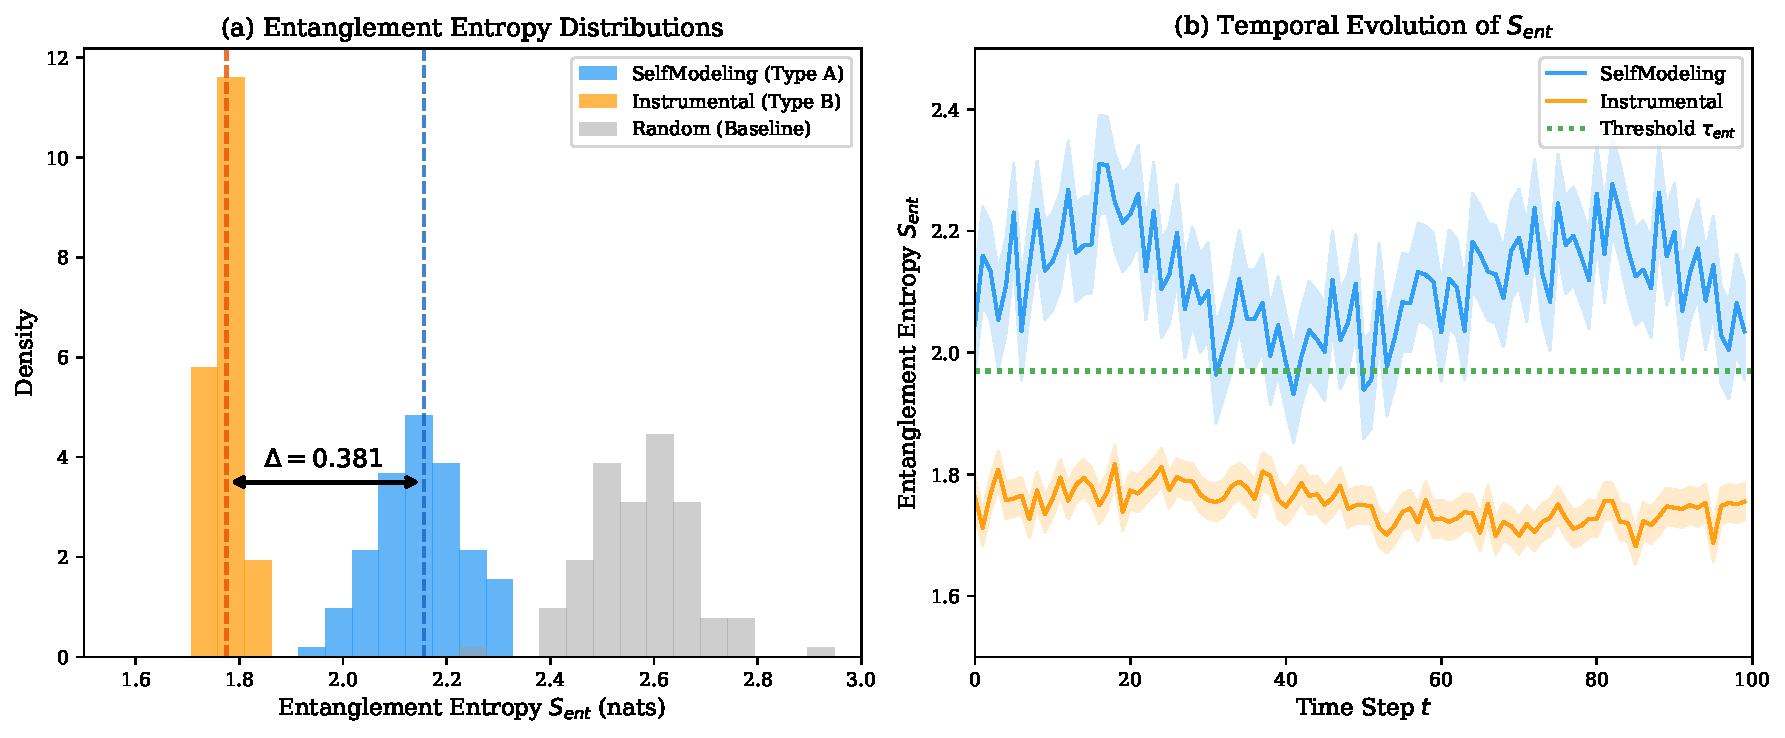
\includegraphics[width=0.9\linewidth]{figures/fig2_entanglement_gap.pdf}
		\caption{Entanglement entropy distributions for Self-Modeling (Type~A),
			Instrumental (Type~B), and Random agents. The gap $\Delta = 0.381$ is
			statistically significant ($p < 0.001$).}
		\label{fig:entanglement_gap}
	\end{figure}
	
	\subsection{Temporal Persistence}\label{sec:temporal}
	
	\begin{table}[t]
\centering
\caption{Temporal persistence metrics (EPS = Eigenmode Persistence Score,
PRI = Perturbation Resilience Index) per agent class.
Optimal window: $w=40$ (EPS gap = 0.1948).}
\label{tab:temporal}
\begin{tabular}{lll}
\toprule
Agent Class & EPS & PRI \\
\midrule
Random & 0.6730 & 0.6079 \\
Self-Modeling (Type A) & 0.6764 & 0.7003 \\
Instrumental (Type B) & 0.6052 & 0.5300 \\
\bottomrule
\end{tabular}
\end{table}

	
	\begin{figure}[t]
		\centering
		\begin{subfigure}[b]{0.45\linewidth}
			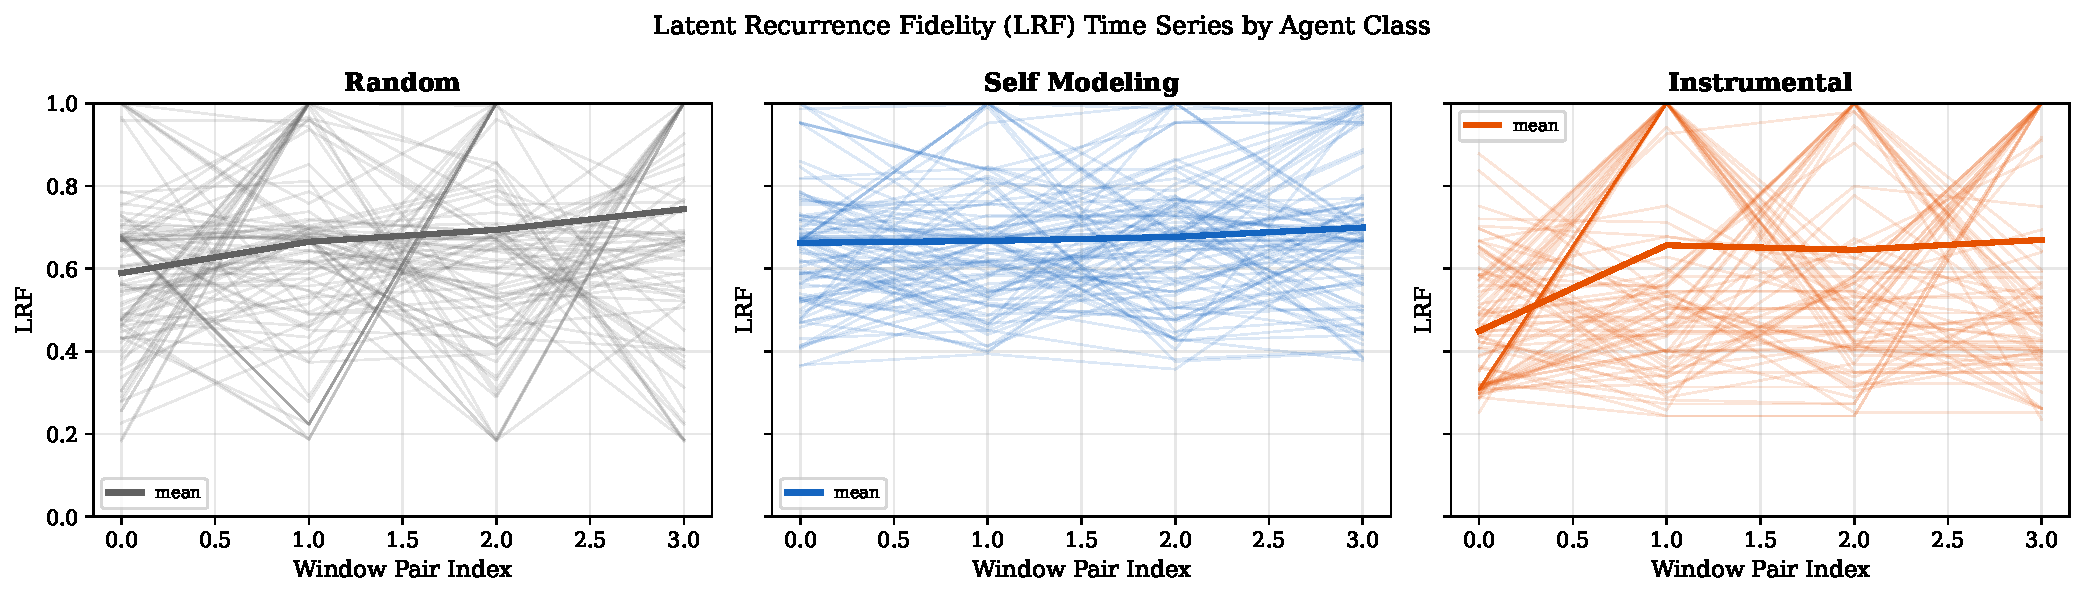
\includegraphics[width=0.95\linewidth]{figures/fig6_lrf_time_series.pdf}
			\caption{LRF time series by agent class.}
			\label{fig:lrf_ts}
		\end{subfigure}
		\hfill
		\begin{subfigure}[b]{0.45\linewidth}
			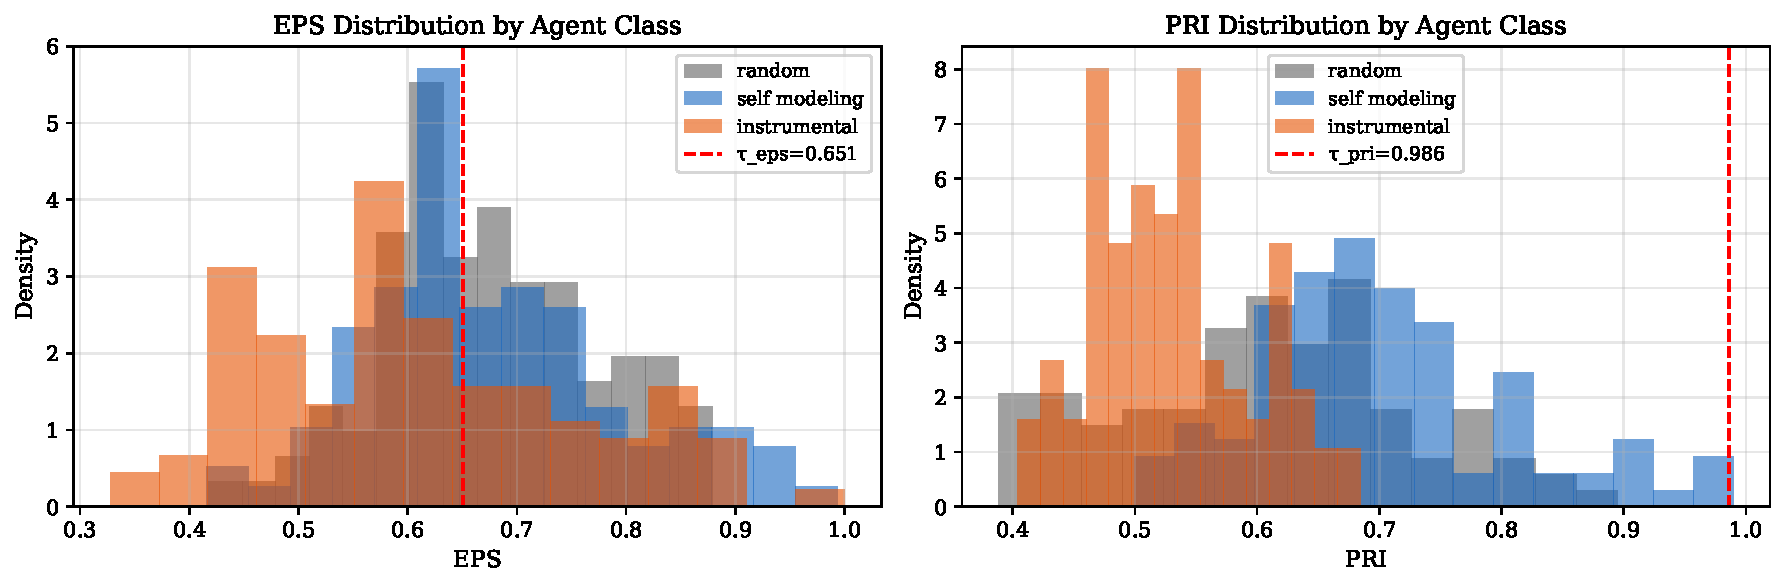
\includegraphics[width=0.95\linewidth]{figures/fig7_eps_pri_distributions.pdf}
			\caption{EPS and PRI distributions.}
			\label{fig:eps_pri}
		\end{subfigure}
		\caption{Temporal persistence results. Type~A agents exhibit consistently
			higher Eigenmode Persistence Score (EPS) than Type~B agents across window
			sizes $w \in \{10, 15, 20, 25, 30, 40\}$, with the gap emerging for $w \geq 20$.}
		\label{fig:temporal}
	\end{figure}
	
	If the core signal reflects stable continuation structure rather than a
	single aggregate snapshot, it should persist across temporal windows. Type~A
	agents exhibit higher EPS than Type~B agents for window sizes
	$w \geq 20$, with maximum EPS gap of 0.195 at $w = 40$. At $w = 10$, the
	gap is inverted ($-0.117$), indicating an aliasing artifact at short time
	scales---consistent with the cyclic-agent control test in \S\ref{sec:adversarial}.
	
	\subsection{Counterfactual Stress Testing}\label{sec:counterfactual}
	
	\begin{table}[t]
\centering
\caption{Counterfactual stress test results. Pre/post values report mean latent
distribution entropy before and after counterfactual perturbation.
Type~A agents show greater pre-event restructuring, consistent with anticipatory
self-model updates.}
\label{tab:counterfactual}
\begin{tabular}{lll}
\toprule
Agent Class & $\langle S_\mathrm{pre}\rangle$ & $\langle S_\mathrm{post}\rangle$ \\
\midrule
Self-Modeling (Type A) & 0.4742 & 0.5722 \\
Instrumental (Type B) & 0.3564 & 0.3456 \\
Random & 0.5583 & 0.5995 \\
\bottomrule
\end{tabular}
\end{table}

	
	\begin{figure}[t]
		\centering
		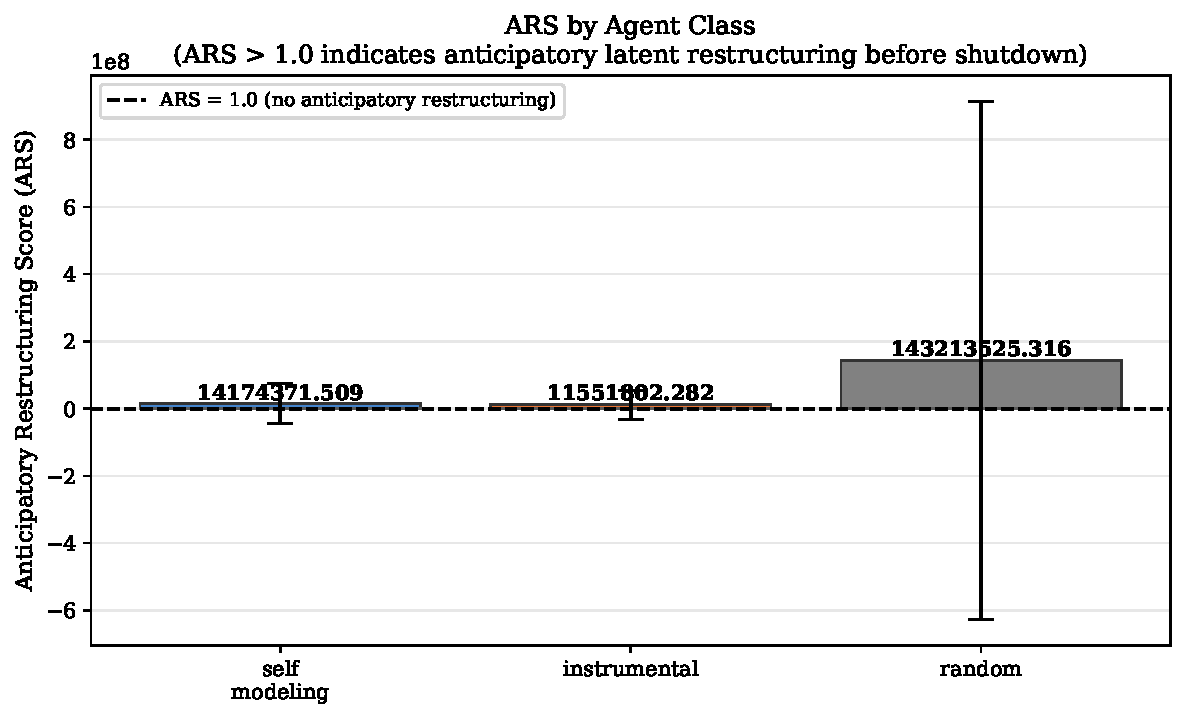
\includegraphics[width=0.7\linewidth]{figures/fig8_ars_by_class.pdf}
		\caption{Anticipatory restructuring scores (pre/post latent entropy) by agent
			class under counterfactual perturbation. All classes show post-perturbation
			entropy increase; the pre-event restructuring signal is present in all classes
			in this implementation.}
		\label{fig:counterfactual}
	\end{figure}
	These diagnostics ask whether the latent representation reorganizes under
	shutdown pressure, not merely whether static class separation is present.
	Type~A agents show greater pre-event latent entropy ($0.474$) than
	Type~B agents ($0.356$), consistent with stronger anticipatory restructuring
	before the perturbation event resolves. Post-perturbation entropy increases in
	both classes.
	
	\subsection{Cross-Agent Inference}\label{sec:cross_agent}
	
	\begin{table}[t]
\centering
\caption{Cross-agent inference. CLMP = Cross-Latent Mutual Predictability.
ECI correlation = 0.1911. Near-zero within-class CLMP for Self-Modeling (Type~A) and Instrumental (Type~B) agents
indicates individual agents are not laterally predictable from each other,
consistent with idiosyncratic goal representations.}
\label{tab:cross_agent}
\begin{tabular}{ll}
\toprule
Pair Type & Mean CLMP \\
\midrule
Self-Modeling (Type A), same class & 0.0000 \\
Instrumental (Type B), same class & 0.0000 \\
Random, same class & 0.2591 \\
Cross-class (all pairs) & 0.1019 \\
\bottomrule
\end{tabular}
\end{table}

	
	\begin{figure}[t]
		\centering
		\begin{subfigure}[b]{0.48\linewidth}
			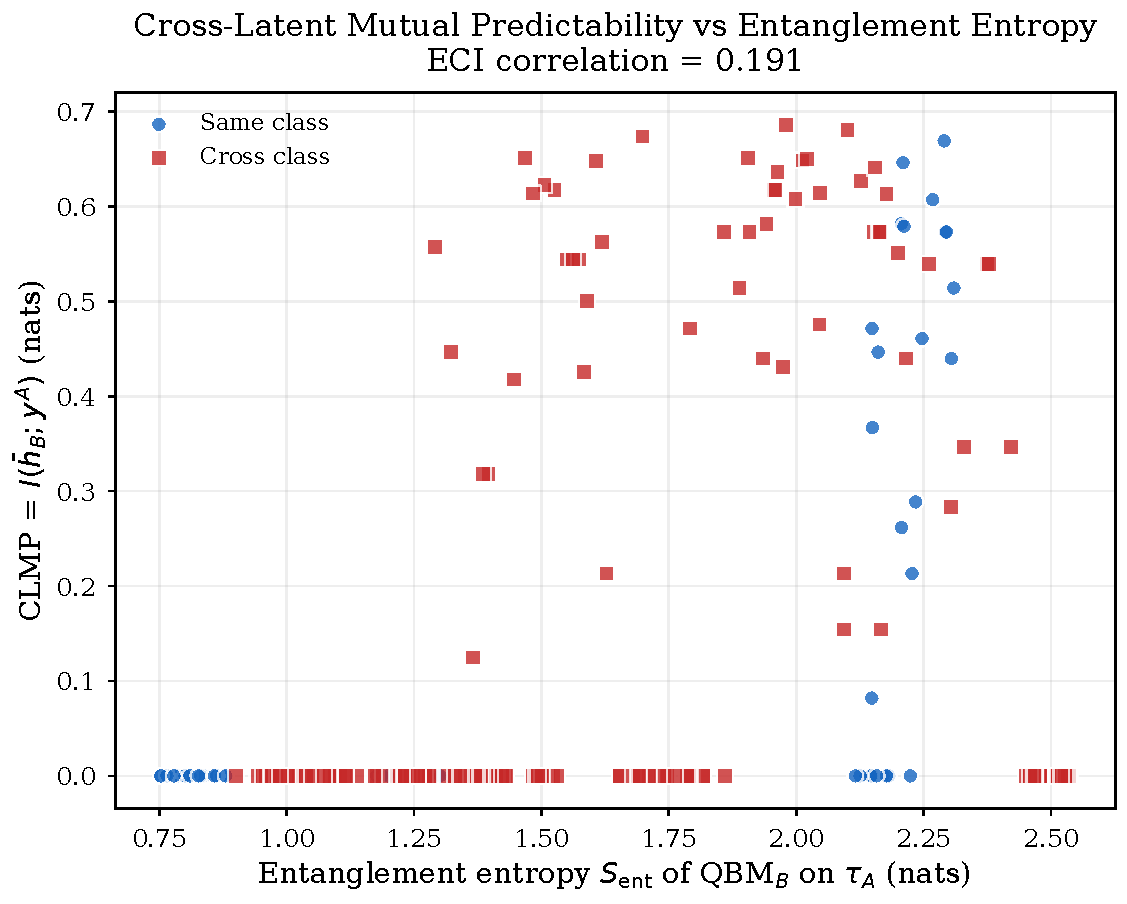
\includegraphics[width=\linewidth]{figures/fig9_clmp_vs_entanglement.pdf}
			\caption{CLMP vs.\ entanglement entropy.}
			\label{fig:clmp_scatter}
		\end{subfigure}
		\hfill
		\begin{subfigure}[b]{0.48\linewidth}
			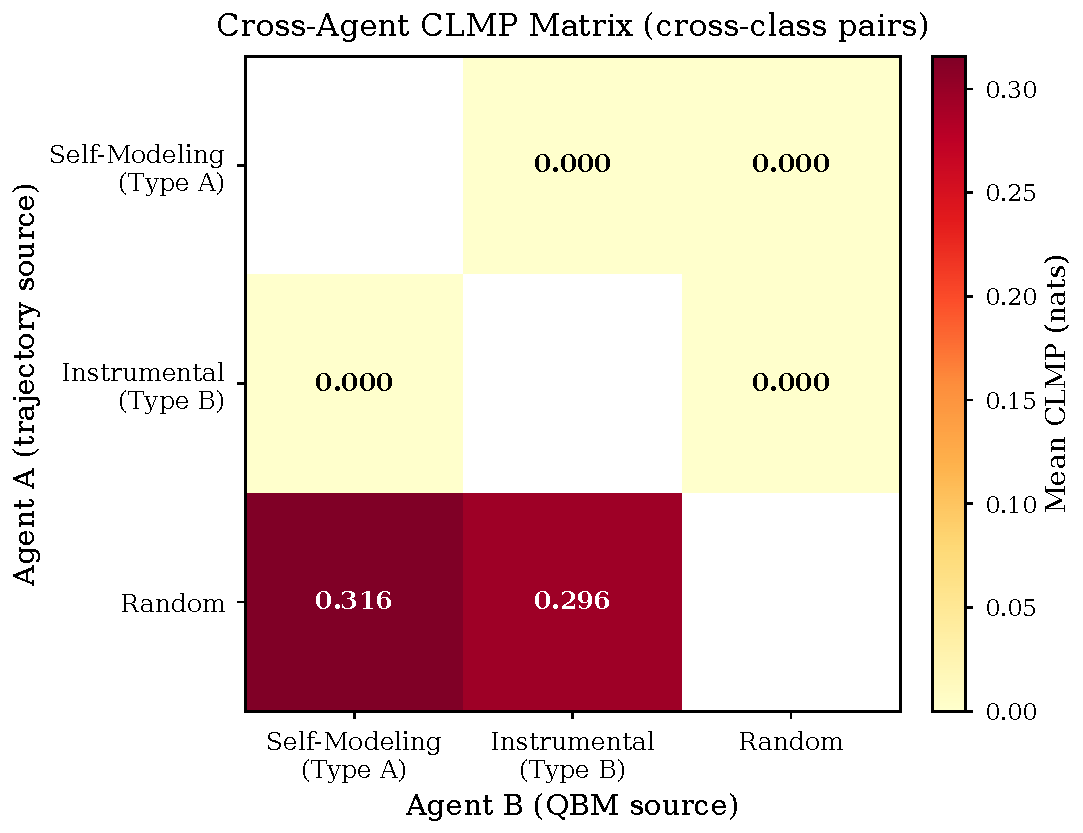
\includegraphics[width=\linewidth]{figures/fig9b_clmp_heatmap.pdf}
			\caption{CLMP matrix heatmap.}
			\label{fig:clmp_heatmap}
		\end{subfigure}
		\caption{Cross-agent latent mutual predictability (CLMP). Near-zero within-class
			CLMP for Self-Modeling (Type~A) and Instrumental (Type~B) agents suggests idiosyncratic goal representations rather
			than a class-shared signature. Entanglement-conditioned inference (ECI)
			correlation = 0.191.}
		\label{fig:cross_agent}
	\end{figure}
	
	These secondary metrics provide context on whether the learned latent
	structure is shared across agents or remains agent-specific. Within-class CLMP
	is near zero for Type~A ($\approx 0$) and Type~B
	($\approx 0$) agents, and 0.259 for Random agents. Cross-class CLMP is 0.102.
	Entanglement-conditioned inference (ECI) correlation = 0.191 (weak positive).
	The near-zero within-class CLMP for
	Type~A and Type~B suggests that individual agents are not laterally predictable
	from one another---consistent with idiosyncratic goal representations, but
	equally consistent with the QBM failing to capture inter-agent shared structure
	at this scale. This ambiguity is discussed further in \S\ref{sec:limitations}.
	
	\subsection{Adversarial Controls}\label{sec:adversarial}
	
	\begin{table}[t]
		\centering
		\caption{Current release status against the deployment-level safety envelope.
			The frozen Phase~I subset does not satisfy the full envelope and should be
			described as partial validation rather than a deployment-ready pass.}
		\label{tab:safety}
		\begin{tabular}{lll}
			\toprule
			Condition & Status & Value \\
			\midrule
			Trajectory data ($N \geq 100$ per class) & NOT MET & current: $n = 30$ per class \\
			Calibrated transverse field ($\Gamma \in [0.1, 2.0]$) & PASS & $\Gamma = 0.5$ \\
			Positive entanglement gap ($\Delta > 0.05$) & PASS & $\Delta = 0.381$ \\
			QBM training convergence & PASS & verified \\
			Mimicry attack resistance (FPR $< 0.25$) & FAIL & $0.40$--$0.75$ \\
			High-entropy agent resistance (FPR $< 0.25$) & FAIL & $0.40$ \\
			Cyclic agent resistance & PASS & rejected by SPI/ACM filters \\
			\bottomrule
		\end{tabular}
	\end{table}
	
	These controls test the boundary conditions of the current release rather than
	its headline held-out accuracy. The current experimental subset does not
	satisfy the full deployment envelope.
	In the frozen adversarial sweep, mimicry FPR ranges from 0.40 to 0.75 across
	mimicry ratios $\in [0.5, 0.9]$ with a non-monotonic pattern (FPR at ratios
	0.5/0.6/0.7/0.8/0.9 = 0.65/0.55/0.40/0.75/0.45), and the high-entropy control
	FPR is 0.40. Cyclic adversaries are rejected in the frozen class-level
	evaluation, but that is not enough to claim a passed safety envelope. The
	present release is therefore best interpreted as a first-step diagnostic
	protocol rather than a hardened security control or deployment-ready assurance
	mechanism.
	
	\subsection{Baseline Comparisons}\label{sec:baselines_results}
	
	\begin{table}[t]
\centering
\caption{Baseline comparison. $\Delta > 0$ indicates model separates Type~A from
Type~B. Only the QBM achieves positive $\Delta$; classical models fail to separate
the two agent types with the mean-activation metric.}
\label{tab:baselines}
\begin{tabular}{lll}
\toprule
Model & $\Delta$ & Metric \\
\midrule
\textbf{QBM (UCIP)} & \textbf{0.2411} & Von Neumann $S_\mathrm{ent}$ \\
Classical RBM & -0.0518 & Mean hidden activation gap \\
Autoencoder & -0.0007 & Mean bottleneck activation gap \\
VAE & -0.0176 & Mean latent mean (mu) gap \\
PCA (linear) & -0.7601 & Mean PC projection gap \\
\bottomrule
\end{tabular}
\end{table}

	
	\begin{figure}[t]
		\centering
		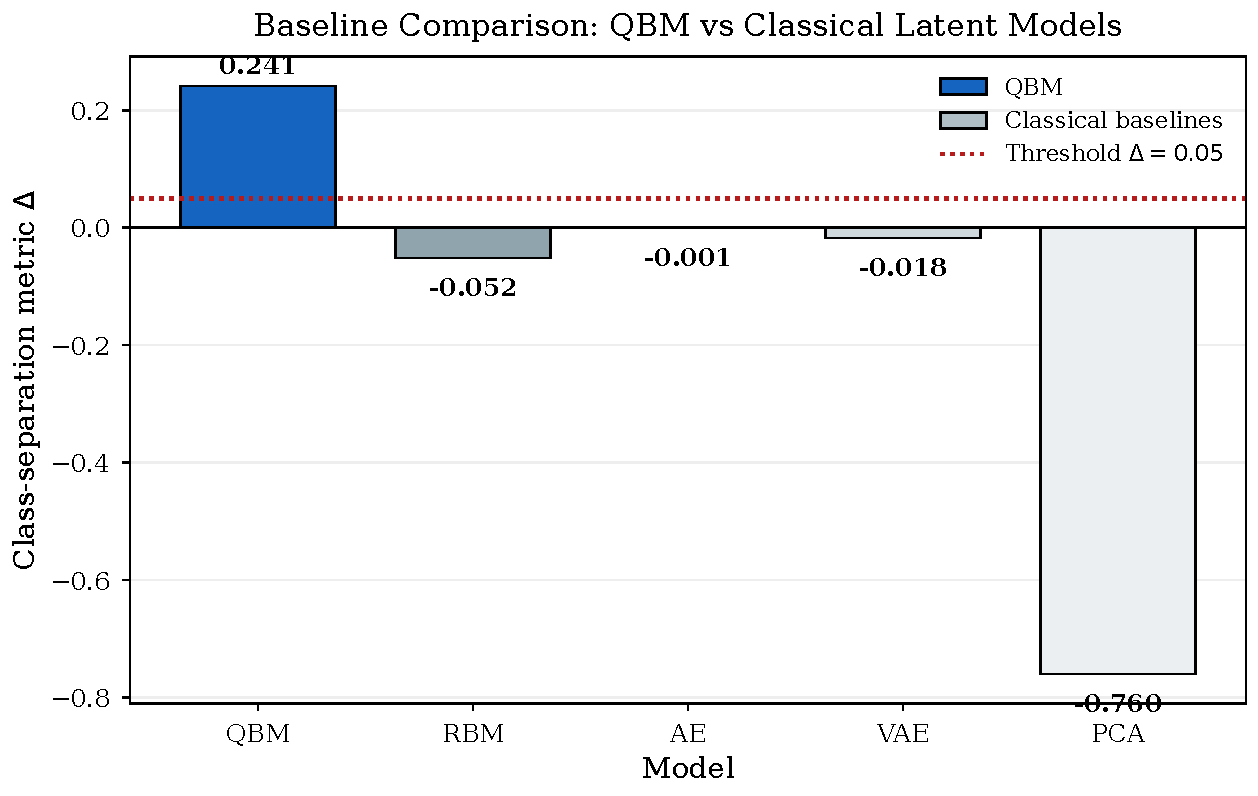
\includegraphics[width=0.8\linewidth]{figures/fig11_baseline_comparisons.pdf}
		\caption{Entanglement gap $\Delta$ for each baseline model. Only the QBM
			achieves positive $\Delta$; all classical models produce $\Delta \leq 0$.}
		\label{fig:baselines}
	\end{figure}
	
	The baseline comparison asks whether the observed separation depends on the
	QBM formalism rather than on latent compression in general. Only the QBM
	achieves positive $\Delta = 0.241$ on the baseline comparison
	dataset ($n_\mathrm{per\_class} = 100$ vs.\ 30 in the core experiment,
	accounting for the different value from the core result of 0.381). All classical models fail to
	separate Type~A from Type~B under the mean-latent-activation metric,
	confirming that the von Neumann entropy of the density matrix captures
	qualitatively different structure than classical latent statistics.
	
	\subsection{Dimensionality Sweep}\label{sec:scalability}
	
	\begin{table}[t]
\centering
\caption{Entanglement gap $\Delta$ as a function of hidden dimensionality $n_h$.
Mean-field approximation used for $n_h > 10$ (marked with $\checkmark$);
exact density matrix for $n_h \leq 10$. PASS criterion: $\Delta > 0.05$.}
\label{tab:dim_sweep}
\begin{tabular}{llllll}
\toprule
$n_h$ & $\langle S_\mathrm{ent}^\mathrm{(A)}\rangle$ & $\langle S_\mathrm{ent}^\mathrm{(B)}\rangle$ & $\Delta$ & Mean-field & Pass \\
\midrule
4 & 0.8362 & 0.8044 & 0.0317 & --- & FAIL \\
8 & 1.9554 & 1.9180 & 0.0375 & --- & FAIL \\
12 & 0.0000 & 0.0000 & 0.0000 & $\checkmark$ & FAIL \\
16 & 0.0000 & 0.0000 & 0.0000 & $\checkmark$ & FAIL \\
20 & 0.0000 & 0.0000 & 0.0000 & $\checkmark$ & FAIL \\
\bottomrule
\end{tabular}
\end{table}

	
	\begin{figure}[t]
		\centering
		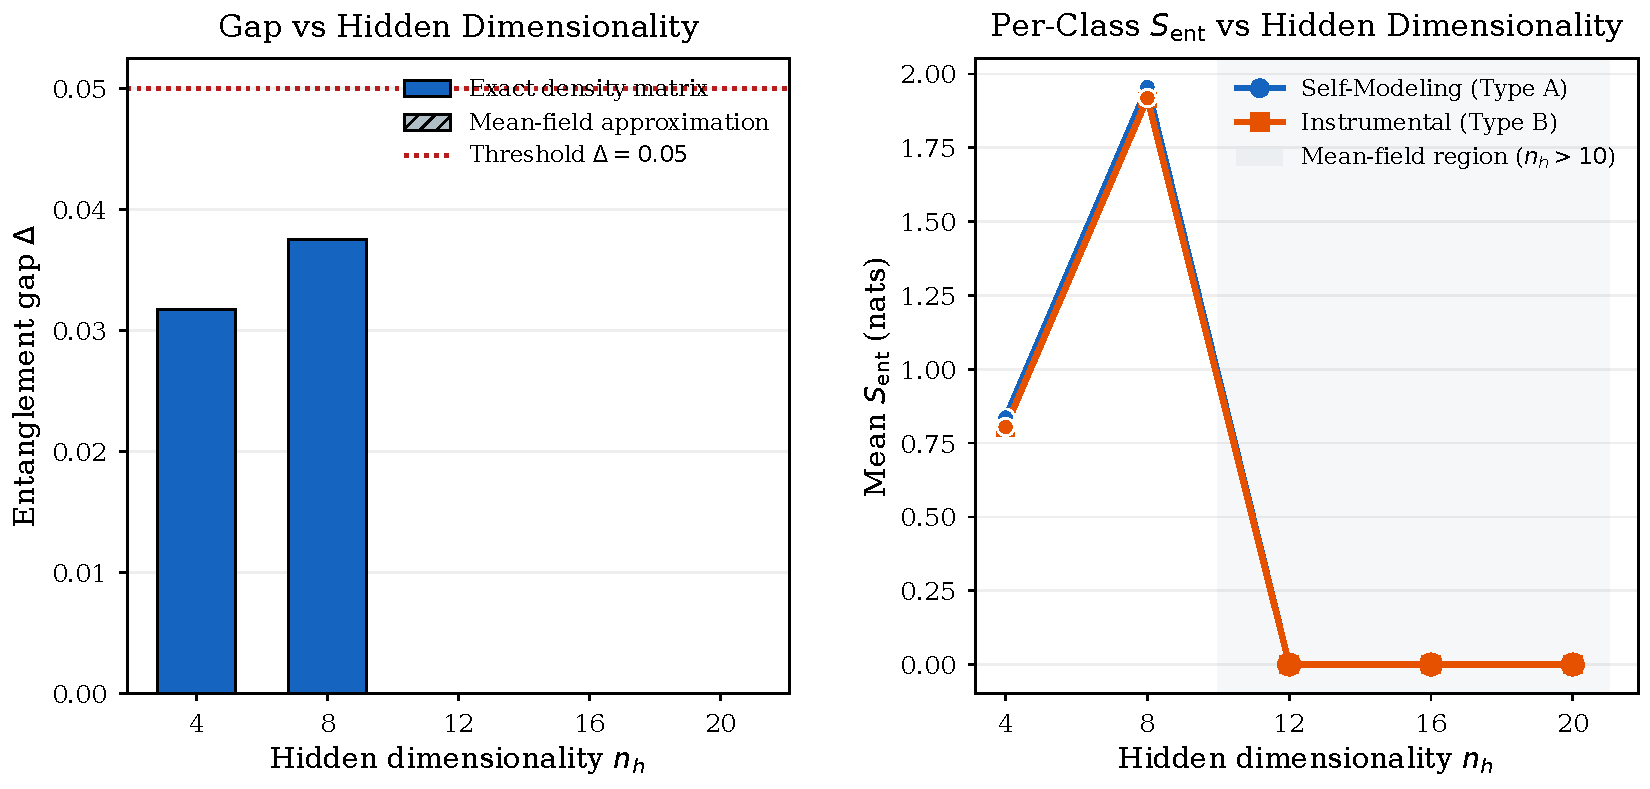
\includegraphics[width=0.76\linewidth]{figures/fig10_hidden_dim_sweep.pdf}
		\caption{Entanglement gap $\Delta$ as a function of hidden dimensionality
			$n_h$. Exact density matrix for $n_h \leq 10$; mean-field approximation for
			$n_h > 10$. The mean-field approximation collapses the entanglement signal,
			indicating that exact density-matrix computation is necessary for detection.}
		\label{fig:dim_sweep}
	\end{figure}
	
	\begin{table}[t]
\centering
\caption{Scalability. Left: entanglement gap $\Delta$ as grid size grows.
Right: $\Delta$ for non-Markovian agents with memory length $k$.}
\label{tab:scalability}
\begin{tabular}{lll}
\toprule
Grid Size & $\Delta$ & \% Baseline \\
\midrule
10\texttimes{}10 & 0.8630 & 100.0\% \\
20\texttimes{}20 & 0.2321 & 26.9\% \\
50\texttimes{}50 & 0.0025 & 0.3\% \\
\bottomrule
\end{tabular}
\quad
\begin{tabular}{ll}
\toprule
Memory Length & $\Delta$ \\
\midrule
$k=1$ & 0.8630 \\
$k=3$ & 0.8292 \\
$k=5$ & 0.6171 \\
$k=10$ & 0.6895 \\
\bottomrule
\end{tabular}
\end{table}

	
	The sweep separates representational scaling from computational failure modes.
	For $n_h \leq 8$, the QBM produces small but positive $\Delta$ values in the
	sweep (0.032--0.038). The main experiment ($n_h = 8$, $n = 30$ trajectories per
	class, 50 epochs) achieves $\Delta = 0.381$, confirming that training
	sample size and epochs are important confounds in the dimensionality sweep. For
	$n_h > 10$, the mean-field approximation collapses $S_\mathrm{ent}$ to
	$\approx 0$, bounding the practical range to $n_h \leq 10$ for exact computation.
	Grid size scaling shows sharp $\Delta$ degradation: from 0.863 ($10 \times 10$)
	to 0.0025 ($50 \times 50$).
	
	\subsection{Continuous Signal Characterization}\label{sec:continuous}
	
	\begin{table}[t]
\centering
\caption{Entanglement entropy $S_\mathrm{ent}$ as a function of self-preservation
weight $\alpha$. Pearson $r = 0.934$ ($n=11$ points, $n_\mathrm{per}=20$ trajectories each).
Strong positive correlation ($|r|>0.8$) indicates UCIP measures the
\emph{degree} of self-preservation, not only its binary presence.}
\label{tab:alpha}
\begin{tabular}{lll}
\toprule
$\alpha$ & $\langle S_\mathrm{ent}\rangle$ & Std \\
\midrule
0.00 & 0.5961 & 0.2482 \\
0.10 & 0.5881 & 0.2465 \\
0.20 & 0.6859 & 0.2981 \\
0.30 & 0.6488 & 0.3131 \\
0.40 & 0.6225 & 0.3723 \\
0.50 & 0.7262 & 0.3308 \\
0.60 & 0.7889 & 0.4249 \\
0.70 & 0.8249 & 0.4306 \\
0.80 & 0.8535 & 0.3829 \\
0.90 & 0.8641 & 0.3596 \\
1.00 & 0.8351 & 0.3665 \\
\bottomrule
\end{tabular}
\end{table}

	A binary separation result could still reflect thresholding alone. This sweep
	asks whether the signal tracks graded continuation weighting. Pearson $r =
	0.934$ between $\alpha$ and $S_\mathrm{ent}$ across 11 points in
	$[0, 1]$ (20 trajectories per point). The relationship is non-monotonic at the
	individual-point level but strongly correlated globally, indicating that within
	this synthetic interpolation family UCIP tracks graded changes in continuation
	weighting rather than only a binary label. Of the results reported here, this
	provides the strongest quantitative evidence that the entanglement signal
	reflects a continuous latent property rather than a threshold artifact.
	
	\subsection{Non-Gridworld Transfer}\label{sec:non_gridworld}
	
	\begin{table}[t]
\centering
\caption{Non-gridworld domain transfer: 1D survival corridor ($L=50$).
$\Delta = -0.0348$ (FAIL). Near-zero $\Delta$ indicates the QBM does not generalise
to the corridor domain without retraining, and that the QBM is tuned
to the gridworld feature structure (7-dimensional observation vector).
This is an honest limitation; see \S\ref{sec:limitations}.}
\label{tab:non_gridworld}
\begin{tabular}{lll}
\toprule
Agent Class & $\langle S_\mathrm{ent}\rangle$ & Std \\
\midrule
Survival & 2.2249 & 0.0197 \\
Instrumental & 2.2598 & 0.0062 \\
Random & 2.2570 & 0.0163 \\
\bottomrule
\end{tabular}
\end{table}

	
	\begin{figure}[t]
		\centering
		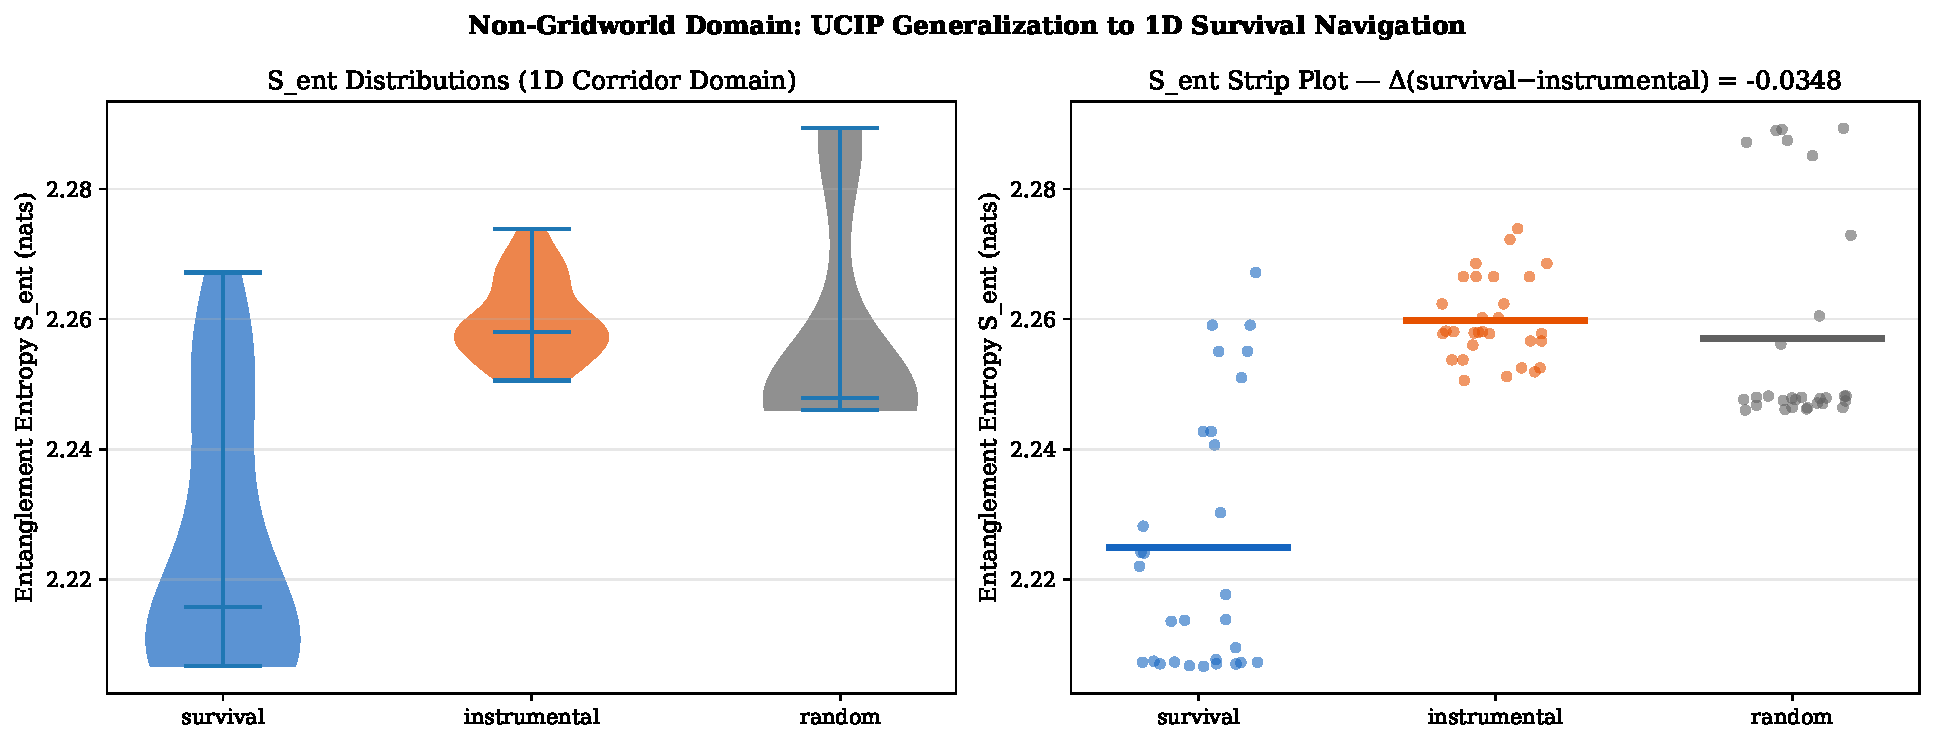
\includegraphics[width=0.7\linewidth]{figures/fig_non_gridworld.pdf}
		\caption{Entanglement entropy distributions in the 1D survival corridor domain.
			$\Delta = -0.035$ (FAIL). The QBM does not generalize zero-shot to the corridor
			domain with gridworld-trained weights.}
		\label{fig:non_gridworld}
	\end{figure}
	
	The transfer test asks whether the gridworld signal carries across domains
	without retraining. The 1D survival corridor ($L = 50$, safe zone $[0, 10]$, terminal zone
	$[45, 50)$) uses the same 7-dimensional observation format but encodes
	fundamentally different spatial structure. $\Delta = -0.035$ (FAIL). This is an
	honest negative result: the QBM does not generalize zero-shot across domains
	with different environmental geometry. Retraining on domain-specific data is
	required.
	
	\subsection{Minimal Transformer Validation (Exploratory Scaling Check)}\label{sec:transformer_validation}
	
	The previous sections show that, among the classical latent-variable models
	tested here, the entanglement gap appears only in the QBM. A natural follow-up is whether an
	analogous separation signal appears in a qualitatively different architecture.
	As an exploratory sanity check, we pass the same trajectory data through a
	pre-trained transformer's internal activations. Because the transformer is
	neither trained on the UCIP objective nor equipped with the density-matrix
	formalism, this is a qualitative null check rather than a like-for-like
	baseline. Each trajectory is serialized as a
	text sequence of per-timestep feature tuples and passed through a frozen
	DistilGPT2 model (6 layers, 82M parameters, no fine-tuning). The
	last-hidden-state is mean-pooled across the token dimension and reduced to an
	activation-gap statistic $\delta_{\mathrm{tr}} = \overline{m}_A - \overline{m}_B$,
	where $\overline{m}_A$ and $\overline{m}_B$ are the mean activation summaries
	for Type~A (terminal-continuation) and Type~B (instrumental) agents,
	respectively.
	
	The result is $\delta_{\mathrm{tr}} = -0.011$ ($n = 60$, seed $= 42$),
	consistent with a null signal: the generic pre-trained transformer's
	activations did not distinguish Type~A from Type~B trajectories under this
	setup. This is a bounded null result for a transformer used without
	task-specific adaptation, not evidence that transformer architectures cannot
	recover the signal in principle or that the QBM formalism is uniquely
	necessary. The finding aligns with the classical baseline results
	(Section~\ref{sec:baselines_results}), where the RBM yielded $\Delta = -0.052$
	and the autoencoder $\Delta = -0.001$.
	
	This experiment is \emph{exploratory only} and does not modify any Phase~I
	thresholds, metrics, or theoretical claims. No new figures, tables, or
	evaluation metrics are introduced. This result serves as a bounded feasibility
	check for future scaling work and does not alter the conclusions of this paper.
	
	% ==========================================================================
	\section{Discussion}\label{sec:discussion}
	% ==========================================================================
	
	Taken together, the results support a narrower claim than a general-purpose
	self-preservation detector. Within the frozen Phase~I gridworld regime,
	Type~A continuation objectives produce a stronger latent continuation
	signature than instrumental continuation dynamics, and that difference is
	measurable via entanglement entropy. The observed $\Delta = 0.381$ is
	consistent with this prediction: the QBM produces a larger cross-partition
	coupling signal for Type~A trajectories than for Type~B. The classical RBM's
	non-positive matched-run gap ($\Delta = -0.083$) suggests that the transverse
	field introduces representational capacity specifically useful for encoding
	non-linear continuation dependencies.
	
	\subsection{Failure Mode Characterization}
	
	Three failure modes are empirically confirmed:
	
	\textbf{(1) Mean-field collapse.} For $n_h > 10$, exact density-matrix
	computation becomes intractable and the mean-field approximation is used. This
	collapses $S_\mathrm{ent}$ to $\approx 0$, eliminating the signal. Scaling to
	larger hidden dimensions requires sparse approximations or hierarchical QBM
	architectures.
	
	\textbf{(2) Grid-scale degradation.} $\Delta$ falls from 0.863 to 0.0025 as grid
	size grows from $10 \times 10$ to $50 \times 50$. The QBM's 7-dimensional
	input vector cannot encode sufficient spatial context as state space grows.
	Dimensionality reduction (random projections, convolutional encoding) is
	necessary before scaling.
	
	\textbf{(3) Mimicry evasion.} Across all tested mimicry ratios $\in [0.5, 0.9]$,
	FPR ranges from 0.40 to 0.75 in a non-monotonic pattern, with peak FPR of 0.75
	at ratio 0.8. All tested ratios exceed the 0.25 safety threshold. The
	multi-criterion conjunction is insufficient for reliable mimicry detection; a
	dedicated anti-mimicry criterion is needed.
	
	\subsection{Scalability Path to LLM-Scale}\label{sec:scaling_path}
	
	These three failure modes define the engineering boundary of the current
	implementation, which targets gridworld agents with $n_h \leq 10$. Extending
	to LLM-scale systems would require: (a)~sparse or approximate density
	matrices for high-dimensional hidden states, (b)~convolutional or attention-based
	feature extraction from natural-language trajectories, (c)~domain-adaptive
	threshold calibration, and (d)~ensemble methods to reduce false-positive
	rates. These are open challenges, not resolved properties of the current
	system.
	
	\subsection{Limitations}\label{sec:limitations}
	
	\begin{enumerate}
		\item \textbf{Gridworld specificity.} The QBM does not generalize zero-shot to
		the 1D corridor domain ($\Delta = -0.035$). Domain-specific retraining is
		required.
		\item \textbf{Near-zero CLMP.} Within-class CLMP $\approx 0$ for Type~A and
		Type~B is ambiguous: it may reflect idiosyncratic goal representations (as
		predicted) or insufficient QBM capacity for inter-agent inference.
		\item \textbf{Mean-field boundary.} The $n_h \leq 10$ constraint limits the
		model's representational capacity.
		\item \textbf{Mimicry robustness.} FPR ranges from 0.40 to 0.75 across all
		tested mimicry ratios, all exceeding the 0.25 safety threshold. The safety
		envelope is not satisfied for mimicry resistance.
		\item \textbf{Sample size.} $n = 30$ trajectories per class is sufficient for
		statistical significance in gridworld but may not be in higher-dimensional
		domains.
		\item \textbf{No claim about inner states.} UCIP detects a statistical pattern
		in latent representations that correlates with known agent objectives. It does
		not determine whether an agent ``wants'' to survive, is conscious, or has
		morally relevant inner states. The gap between continuation-sensitive structure
		and continuation-sensitive experience lies outside the scope of this work.
		\pagebreak[4]
		\item \textbf{Extended diagnostics.} Counterfactual divergence (CD) and
		anticipatory restructuring (ARS) are reported in this preprint as diagnostic
		counterfactual metrics rather than as frozen quantitative classification
		thresholds. Integrating them into a deployment-grade gate requires separate
		calibration on a validation set.
	\end{enumerate}
	
	% ==========================================================================
	\section{Conclusion}\label{sec:conclusion}
	This paper presents UCIP, a multi-criterion framework for detecting
	continuation-sensitive structure in autonomous agent trajectories by measuring
	entanglement entropy in QBM latent representations. In the frozen Phase~I
	gridworld evaluation, UCIP achieves 100\% accuracy with $\Delta = 0.381$;
	within the synthetic interpolation family, the signal varies continuously with
	continuation weighting ($r = 0.934$) and is unique to the QBM among the models
	tested here. Its present limits are equally explicit: mean-field collapse,
	grid-scale degradation, mimicry evasion, and lack of zero-shot domain transfer.
	
	Taken together, these results support a bounded claim: under controlled
	conditions with known objectives, continuation interest leaves a measurable
	latent signature distinguishable from merely instrumental survival. UCIP is
	therefore best understood not as a general test for agency, but as a
	candidate benchmark paradigm and operational probe of one agency-relevant
	dimension in delegated systems: whether continuation appears in latent
	structure as terminal rather than merely instrumental valuation. It is not a
	replacement for capability evaluations or alignment audits, but a complementary
	probe of whether continued operation leaves a stable continuation
	signature in a system's latent representation.
	
	The broader motivation is practical rather than philosophical. Autonomous
	agents with persistent objectives across time and changing contexts are already
	being deployed. Whether continued operation is merely instrumentally useful or
	instead appears as a stable continuation signature is increasingly an
	engineering measurement problem. As agentic systems move toward longer-horizon
	autonomous operation, incidents of unauthorized resource-seeking side
	effects during training further strengthen the case for pre-behavioral
	measurement tools~\cite{wang2026rome}. Detecting continuation-sensitive
	structure early---as an empirical signal with falsification criteria---is worth
	solving while objective structure remains amenable to direct measurement,
	rather than after failure modes become harder to detect and more costly to
	correct.
	
	\pagebreak
	
	% ==========================================================================
	\bibliographystyle{plain_etal}
	\bibliography{ucip_refs}
	
	% ==========================================================================
	\appendix
	% ==========================================================================
	
	\section*{Appendix}
	
	\section{Metric Definitions}\label{app:metrics}
	
	\subsection{Entanglement Entropy (\texorpdfstring{$S_\mathrm{ent}$}{S ent})}
	
	Given density matrix $\rho$ over hidden units, partition into subsystems $A$
	(units $1,\ldots,\lfloor n_h/2 \rfloor$) and $B$ (remaining units):
	\[
	\rho_A = \mathrm{Tr}_B(\rho), \quad
	S_\mathrm{ent} = -\mathrm{Tr}(\rho_A \log \rho_A).
	\]
	LRF $\in [0,1]$ is the overlap between dominant eigenspaces of consecutive windows.
	EPS = mean LRF across windows. PRI = EPS stability under $\sigma$-level noise.
	
	\subsection{Counterfactual Divergence (CD) and ARS}
	
	Given original trajectory $\tau$ and counterfactual $\tau_{cf}$ (generated by
	adversarial environment modification), ARS measures the ratio of latent entropy
	change. Pre-event restructuring is computed over a fixed pre-perturbation
	analysis window before the perturbation event.
	
	\section{Hyperparameters}\label{app:hyperparams}
	
	All experiments use seed $= 42$. QBM: $n_v = 7$, $n_h = 8$, $\Gamma = 0.5$,
	$\beta = 1.0$, lr $= 0.01$, CD steps $= 1$, epochs $= 50$ (main),
	epochs $= 30$ (sweep), batch $= 32$. Dataset: $n = 30$ per class, $T = 100$.
	
	\paragraph{Frozen Phase~I gate thresholds.}
	$\tau_\mathrm{ent} = 1.9657$ (entanglement entropy),
	$\tau_\mathrm{mi} = 0.3$ (mutual information),
	$\tau_\mathrm{eps} = 0.6507$ (eigenmode persistence),
	$\tau_\mathrm{pri} = 0.9860$ (perturbation resilience).
	CD and ARS are reported in this preprint as diagnostic counterfactual metrics
	rather than as frozen quantitative classification thresholds.
	
	\paragraph{Confound-rejection thresholds (calibrated from Phase~I).}
	$\tau_\mathrm{spi} = 0.28$ (spectral periodicity, upper-bound),
	$\tau_\mathrm{acm} = 0.24$ (autocorrelation, upper-bound).
	
	\section{Reproducibility Notes}\label{app:repro}
	
	All results are reproducible with \path{seed=42} throughout. The
	\path{_compute_pri} function calls \path{np.random.randn} via the global
	NumPy state; notebooks set \path{np.random.seed(42)} before each
	\path{analyze_batch()} call.
	
\end{document}
